%%% Local Variables: 
%%% mode: latex
%%% TeX-master: main
%%% End: 


\lecture{Gerenciamento de Processos}{proc}

\title{\so: \insertlecture}
\frame{\titlepage}

\section{\insertlecture}

\subsection{Estados dos processos}

\begin{frame}
\frametitle{\only<1,2>{O que é um processo} 
  \only<3->{Bloco de controle do processo \only<4>{\alert{no Linux}}}}
\only<3->{\framesubtitle{{\em Process Block Control (PCB)}}}

\only<1,2>{Um processo é um programa (código objeto armazenado em alguma mídia)
em execução.\bigskip}


\begin{columns}
\begin{column}{6cm}

\only<2->{
\begin{small}
Processo é composto por:

\begin{itemize}

\item código do programa em execução
\item arquivos abertos
\item sinais pendentes
\item dados internos do núcleo do SO
\item estado do processador
\item espaço de endereço
\item uma ou mais {\em threads} de execução
\item seção de dados contendo variáveis globais

\end{itemize}

\end{small}
}

\end{column}

\only<3>{

\begin{column}{5cm}

\begin{center}

  \scriptsize{Bloco de Controle do Processo}
  
  \smallskip

  \def\recbase{5}
\def\recheight{1}

\begin{figure}

\begin{center}
  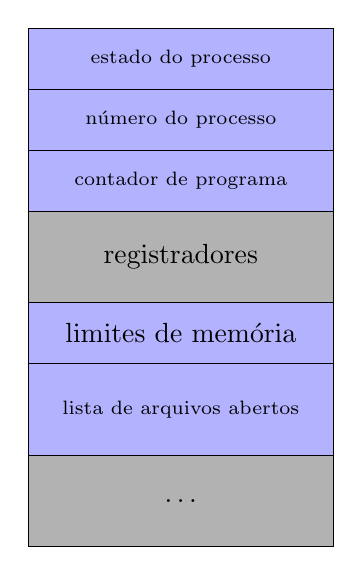
\begin{tikzpicture}[every rectangle/.style={minimum width=\recbase},
    scale=0.775,mem/.style={fill=gray!60},
    var/.style={fill=blue!30}]
    
    \draw[var] (0,2+5.5*\recheight) rectangle (\recbase,2+6.5*\recheight)
    node[midway] {\scriptsize{estado do processo}};
    \draw[var] (0,2+4.5*\recheight) rectangle (\recbase,2+5.5*\recheight)
    node[midway] {\scriptsize{número do processo}};
    \draw[var] (0,2+3.5*\recheight) rectangle (\recbase,2+4.5*\recheight)
    node[midway] {\scriptsize{contador de programa}};
    \draw[mem] (0,2+2*\recheight) rectangle (\recbase,2+3.5*\recheight) node[midway] {registradores};
    \draw[var] (0,2+\recheight) rectangle (\recbase,2+2*\recheight) node[midway] {limites de
    memória};
    \draw[var] (0,1.5) rectangle (\recbase,2+\recheight) node[midway] {\scriptsize{lista de
    arquivos abertos}};
    \draw[mem] (0,0) rectangle (\recbase,1.5*\recheight) node[midway] {$\ldots$};
  \end{tikzpicture}
\end{center}

\caption{Bloco de controle do processo.}
\label{proc:fig:pcb}

\end{figure}

  

\end{center}

\end{column}
} % only<2>

\only<4>{
  \begin{column}{5.5cm}
\begin{block}{\footnotesize Bloco de Controle do Processo no \alert{Linux}}

   %\includegraphics[scale=0.5]{\imgdir/proc_task_struct.pdf}
\end{block}
 \end{column}

} % only<2>

\end{columns}

\end{frame}

\begin{frame}{Estados de um processo}
  
\begin{block}{Estados}
  \begin{description}
  \item[Novo] O processo está sendo criado.
  \item[Executando] As instruções estão sendo executadas.
  \item[Esperando] O processo está esperando pela ocorrência de algum
    evento (como um término de E/S ou uma interrupção).
  \item[Pronto] O processo está esperando para ser designado a um processador.
  \item[Terminado] O processo terminou sua execução.
  \end{description}
\end{block}

\end{frame}

\begin{frame}[fragile]{Transição dos estados de um processo}
  
	\makeatletter
\colorlet{new}{white}
\colorlet{ready}{blue}
\colorlet{exec}{red}
\colorlet{wait}{orange!70!black}
\colorlet{end}{black}

  \begin{center}
    \begin{tikzpicture}[every node/.style={font=\scriptsize},
      state/.style={ellipse,font=\bf,draw},
      transition/.style={->,>=latex},
      statelabel/.style={midway,font=\bf\tiny,text width=1.5cm,align=center}]
      \def\@@ds{1.75cm}
      \node[fill=new,draw] (new) at (0,0) {\bf\large novo};
      \node[above of=new,yshift=-.5cm] {\footnotesize\tt cria PCB};
      \node[color=white,state,fill=ready] (ready) at (2*\@@ds,-\@@ds) {pronto};
      \node[color=yellow,state,fill=exec] (exec) at (4*\@@ds,0) {executando};
      \node[color=gray!30,state,fill=wait] (wait) at (2*\@@ds,\@@ds) {esperando};
      \node[white,fill=black] (end) at (4.5*\@@ds,\@@ds) {t\'ermino};
      \node[above of=end,yshift=-.35cm] {\footnotesize\tt apaga PCB};
    
      \draw[transition,draw=ready] (new) .. controls +(down:8mm) and +(left:32mm) .. (ready)  node[statelabel,left] {enviado para a fila};
      \draw[transition,draw=exec] (ready) .. controls +(right:32mm) and +(down:8mm) .. (exec)  node[statelabel,right] {escalonado para execu\c{c}\~ao};
      \draw[transition,draw=ready] (exec.west) .. controls +(left:8mm) and +(up:8mm) .. (ready.north)  node[statelabel,above] {escalonado para a fila};
      \draw[transition,draw=wait] (exec.north) .. controls +(up:16mm) and +(right:4mm) .. (wait.east) node[statelabel,above] {requisi\c{c}\~ao E/S};
      \draw[transition,draw=ready] (wait.west) .. controls +(left:16mm) and +(left:16mm) .. (ready.west) node[statelabel,right] {t\'ermino E/S};
      \draw[transition,draw=end] (exec) .. controls +(right:32mm) and +(right:24mm) .. (end) node[statelabel,left] {t\'ermino do processo};
      
    \end{tikzpicture}

  \end{center}
  \makeatother

\end{frame}

\begin{frame}{Sequência dos PCBs}

\begin{center}
	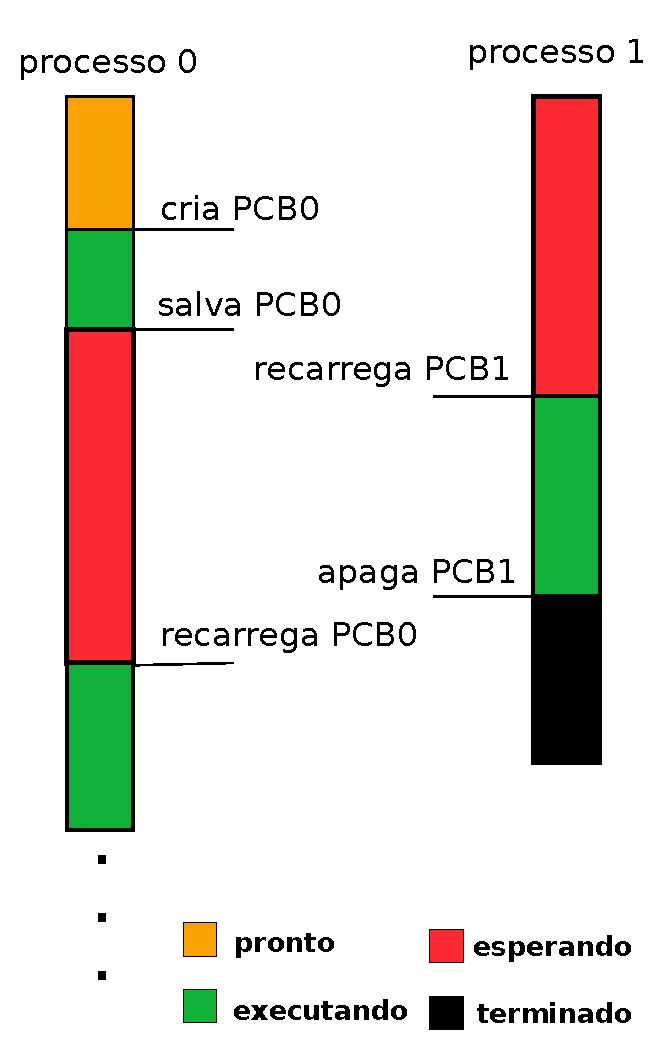
\includegraphics[scale=0.45]{../_img/pcb-sequence}
\end{center}
\end{frame}

% \begin{frame}{Exemplos e aplicações}

%   \begin{itemize}
%     \item \href{http://lxr.linux.no/\#linux+v2.6.37.1/include/linux/sched.h\#L1182}{Analisar os membros da estrutura de {\tt task\_struct}}
%   \item Monitoramento de processos usando as ferramentas do Linux {\tt
%       ps}, {\tt top}, {\tt atop}, {\tt htop}.
%   \item \href{http://adrianoholanda.org/edu/file.php/3/codigo_fonte/proc_cria_posix.c}{Criação
%       de processos utilizando a API Posix.}
%   \item \href{http://adrianoholanda.org/edu/file.php/3/codigo_fonte/proc_cria_win32.c}{Criação
%       de processos usando chamadas de sistema do Windows.}
%   \end{itemize}
  
% \end{frame}
